In this section an STFT will be implemented in Python and tested to check that it fulfils the test criteria specified in chapter \ref{ch3}. This includes creating a spectrogram from the results of the STFT and check if this is consistent with the expected results. The implementation is based on the theory of the discrete STFT described in section \ref{sec:STFT}.

\subsection{Implementation of the STFT and spectrogram}
The implementation of the STFT requires an FFT algorithm and will use the algorithm described in algorithm \ref{FFTalg}.
\\ \\
The STFT will be implemented in Python, and the algorithm for the implementation is seen below in algorithm \ref{STFTalg}.
\begin{algorithm}[H]
\caption{STFT algorithm}
\label{STFTalg}
\begin{algorithmic}[1]
\State $FFTsize=2**N$ \Comment{Length of window and FFT in STFT}
\State $overlap=2$ \Comment{Overlaps of every FFT - 2 is 50\% overlap of adjacent windows}
\State $data = filename.wav$ \Comment{Recording imported as .wav file}\\
\Procedure{Compute STFT}{}
\State $step=FFTsize/overlap$
\State $w=hanning(FFTsize)$ \Comment{Hanning window of length $=FFTsize$}
\For{each $i$ at intervals of $step$ in length of $data-FFTsize$}
\State $stft = array[FFT(w\cdot data[i:i+FFTsize])]$
\EndFor
\State Return $stft$
\EndProcedure
\end{algorithmic}
\end{algorithm}

The algorithm for generating a spectrogram from the STFT is likewise implemented in Python and is seen in algorithm \ref{SPECTROalg}.
\begin{algorithm}[H]
\caption{Generate spectrogram}
\label{SPECTROalg}
\begin{algorithmic}[1]
\State $freq=f_s$ \Comment {Sets sampling frequency of data}
\State $stft=STFT(data)$ \Comment{Perform STFT on $data$}
\State $time=len(data)/freq$ \Comment{Length of data in seconds.}
\State $stft=20\cdot log_{10}(abs(stft.T))$ \Comment{dB gain of transposed $stft$}\\
\State $x=linspace(0,tid,len(X[1]))$ \Comment{Ticks for x-axis}
\State $y=linspace(0,freq/2,len(len(X[0])$ \Comment{Ticks for y-axis}\\
\State $spec=pcolormesh(x,y,X)$ \Comment{Plot amplitudes as colors with positions $(x,y)$}
\State $colorbar(spec)$ \Comment{Legend of colors illustrated as a colorbar}
\end{algorithmic}
\end{algorithm}

\subsection{Validation of the STFT and spectogram}
The validation of the STFT and spectrograms will be done as a whole entity, and the test specification consists of generating a spectrogram from the signal specified in section \ref{sec:STFT_spec}. Figure \ref{fig:test_stft} shows spectrograms of the signal generated with windows of different lengths.
\begin{figure}[H]
\centering
\begin{subfigure}{0.49\textwidth}
\centering
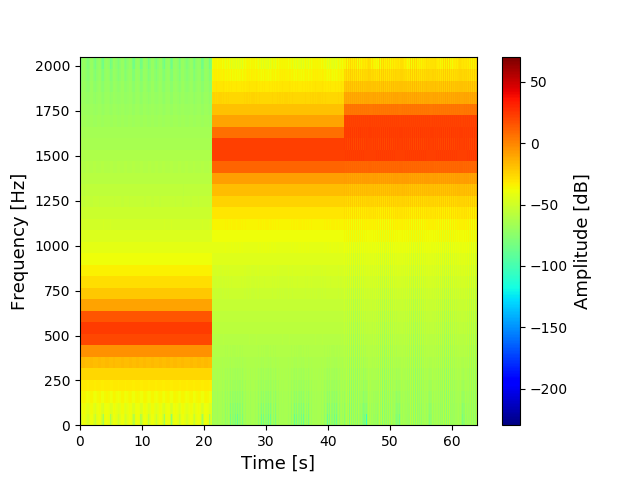
\includegraphics[width=\textwidth]{figures/validation/stft/1.png}
\caption{}
\label{fig:test_stft1}
\end{subfigure}
\begin{subfigure}{0.49\textwidth}
\centering
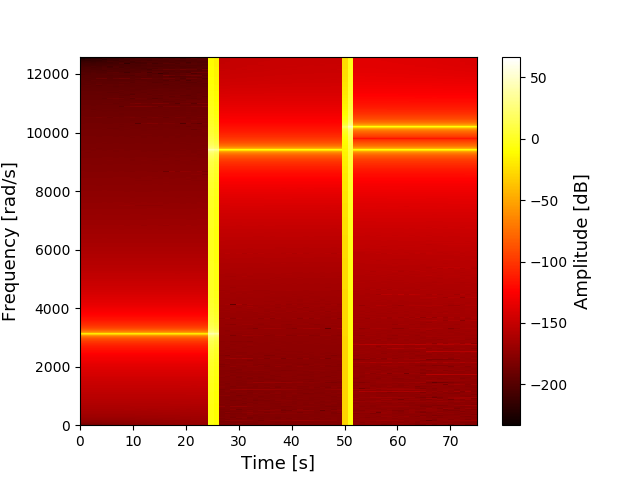
\includegraphics[width=\textwidth]{figures/validation/stft/2.png}
\caption{}
\label{fig:test_stft2}
\end{subfigure}
\caption{\textbf{(a)} Spectrogram of signal in \eqref{eq:SPECTROsignal} generated with window of length $2^{13}=8192$ and overlap of 2. The high spectral and low temporal resolutions follows from a wide window used in the STFT. \textbf{(b)} Spectrogram of signal in \eqref{eq:SPECTROsignal} generated with window of length $2^6=64$ and overlap of 2. The low spectral and high temporal resolutions follow from a narrow window used in the STFT.}
\label{fig:test_stft}
\end{figure}
From figure \ref{fig:test_stft} it is clearly seen how the length of the window in the STFT used for generating the spectrogram affects the resolution in time and frequency. This agrees with Heisenberg's uncertanity principle described in section \ref{sec:heisenberg}, and so there must be made a tradeoff between the two resolutions. For the purpose of this project it is decided to use a window lenght of $2^{11}=2048$ as compromise between the to extreme cases illustrated by figure \ref{fig:test_stft}. \trine{evt. input mht. optimering af fftsize?? heisenberg??\smiley } \\
By figure \ref{fig:test_stft} it is concluded that the implementations of the STFT and spectrogram work as intended. Further optimization is possible through the type window used in the STFT.

\subsection{Variation of windows in STFT}
The STFT uses a window function to taper the segment of the data to be transformed, and different windows produce different results from the STFT. Figure \ref{fig:stft_windows_10000} shows spectrograms of the test signal generated from different windows of length $2^{13}=8192$. Similarly, figure \ref{fig:stft_windows_100} shows spectrograms from STFTs with windows of length $2^6=64$.
\begin{figure}[H]
\centering
\begin{subfigure}{0.49\textwidth}
\centering
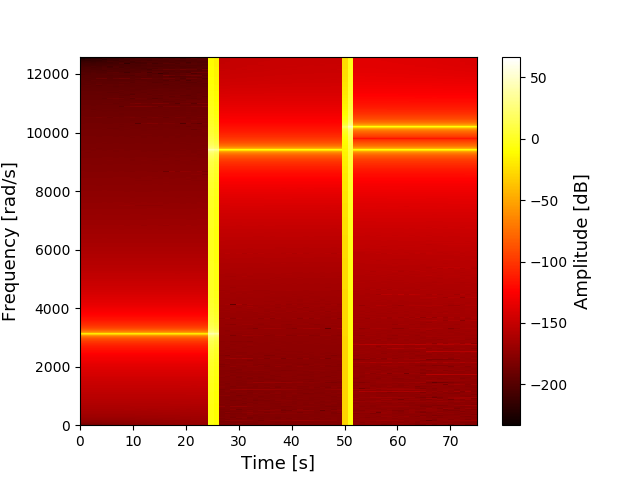
\includegraphics[width=\textwidth]{figures/stft_windows/hanning_10000.png}
\caption{Hanning window.}
\label{fig:stft_hanning}
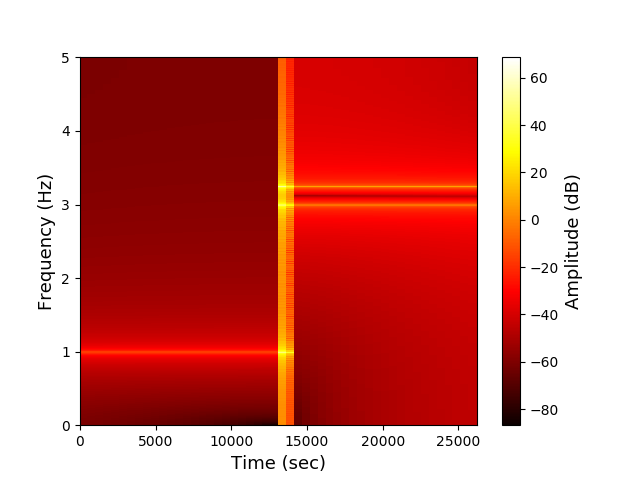
\includegraphics[width=\textwidth]{figures/stft_windows/hamming_10000.png}
\caption{Hamming window.}
\label{fig:stft_hamming}
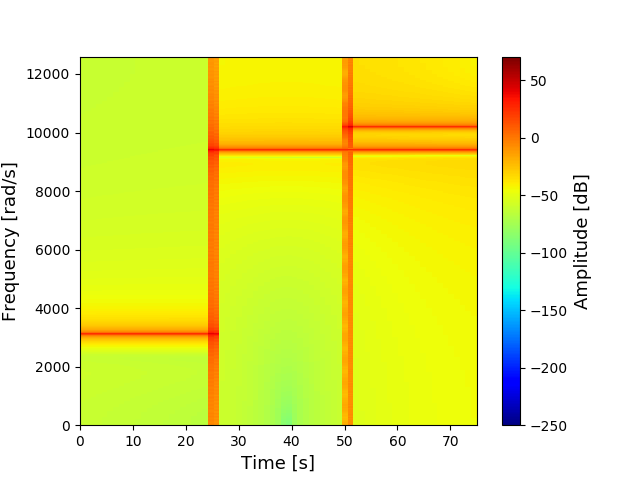
\includegraphics[width=\textwidth]{figures/stft_windows/kaiser/10000/4.png}
\caption{Kaiser window, $\beta=4$.}
\label{fig:stft_kaiser_10000_4}
\end{subfigure}
\begin{subfigure}{0.49\textwidth}
\centering
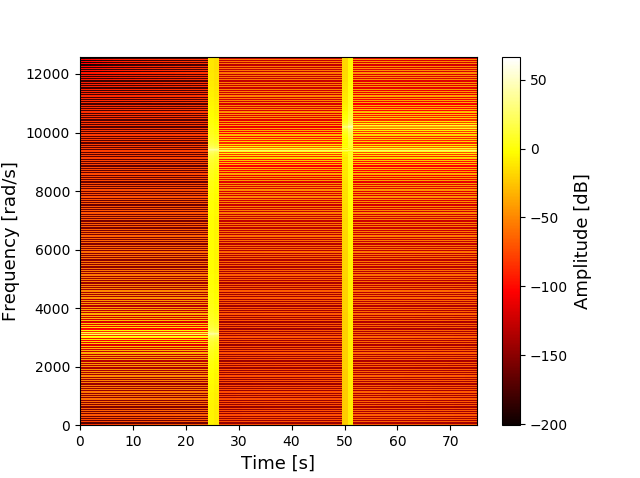
\includegraphics[width=\textwidth]{figures/stft_windows/bartlett_10000.png}
\caption{Bartlett window.}
\label{fig:stft_bartlett}
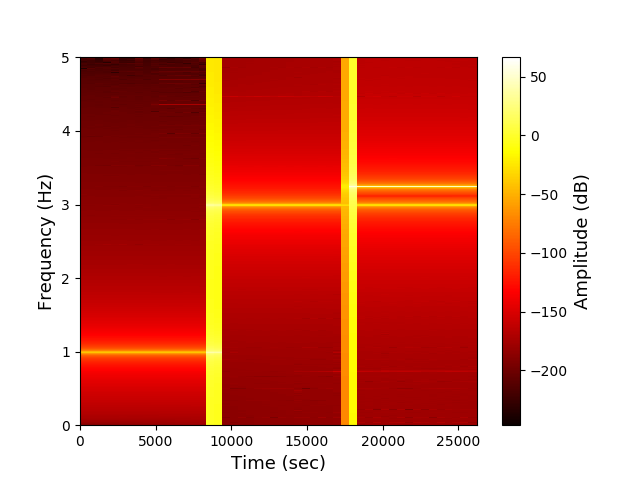
\includegraphics[width=\textwidth]{figures/stft_windows/blackman_10000.png}
\caption{Blackman window.}
\label{fig:stft_blackman}
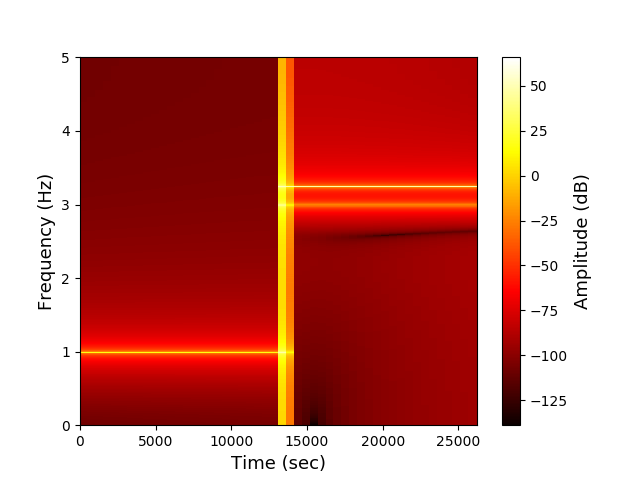
\includegraphics[width=\textwidth]{figures/stft_windows/kaiser/10000/10.png}
\caption{Kaiser window, $\beta=10$.}
\label{fig:stft_kaiser_10000_10}
\end{subfigure}
\caption{Spectrograms generated with different windows of length $2^{13}$ and with overlap of 2.}
\label{fig:stft_windows_10000}
\end{figure}
\begin{figure}[H]
\centering
\begin{subfigure}{0.49\textwidth}
\centering
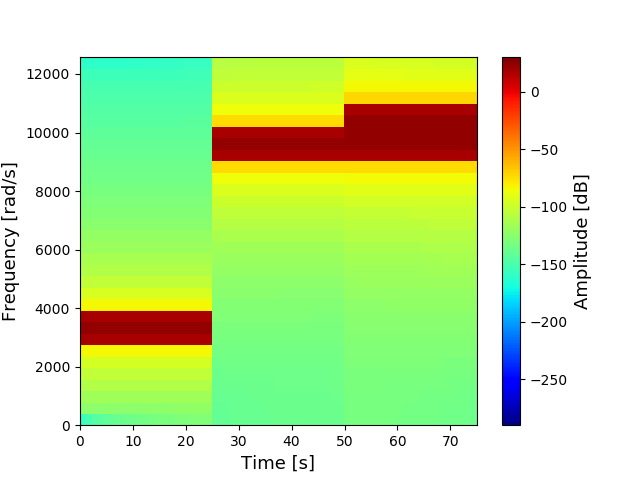
\includegraphics[width=\textwidth]{figures/stft_windows/100/hanning.png}
\caption{Hanning}
\label{fig:stft_hanning_100}
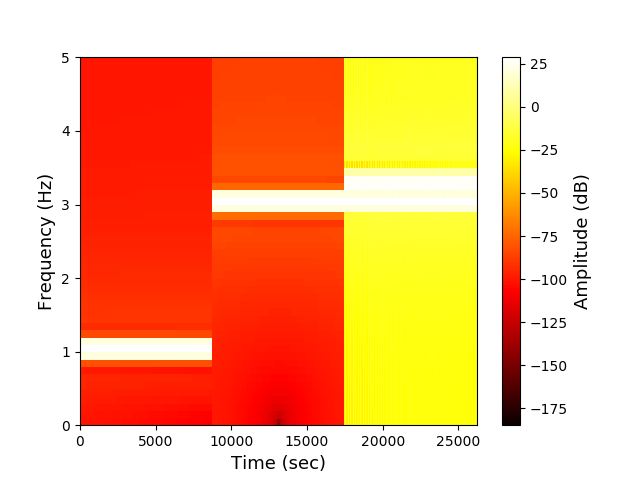
\includegraphics[width=\textwidth]{figures/stft_windows/100/hamming.png}
\caption{Hamming window.}
\label{fig:stft_hamming_100}
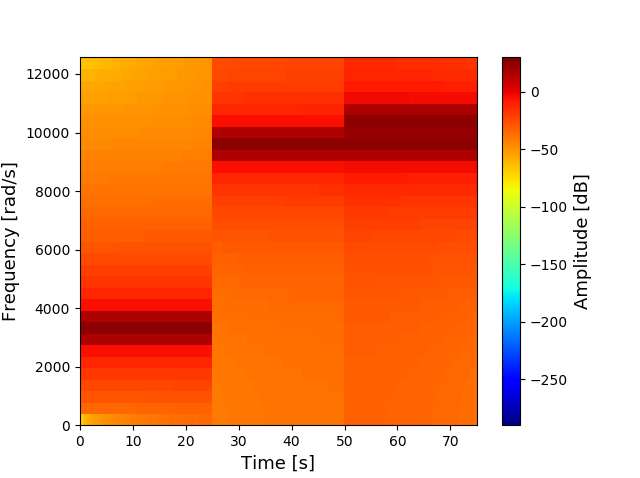
\includegraphics[width=\textwidth]{figures/stft_windows/100/kaiser_4.png}
\caption{Kaiser window, $\beta=4$.}
\label{fig:stft_kaiser_100_4}
\end{subfigure}
\begin{subfigure}{0.49\textwidth}
\centering
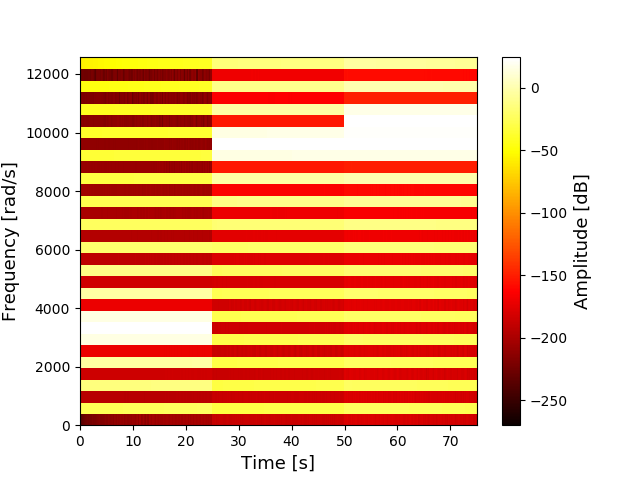
\includegraphics[width=\textwidth]{figures/stft_windows/100/bartlett.png}
\caption{Bartlett window.}
\label{fig:stft_bartlett_100}
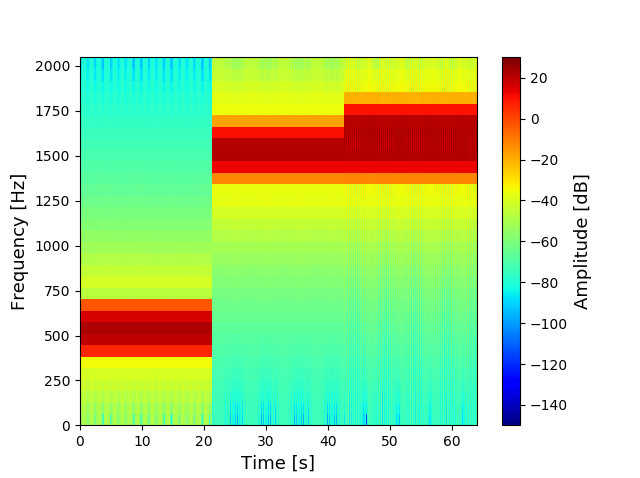
\includegraphics[width=\textwidth]{figures/stft_windows/100/blackman.png}
\caption{Blackman window.}
\label{fig:stft_blackman_100}
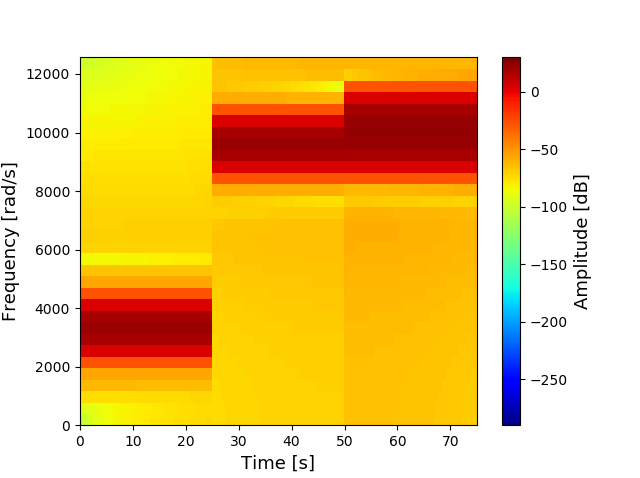
\includegraphics[width=\textwidth]{figures/stft_windows/100/kaiser_10.png}
\caption{Kaiser window, $\beta=10$.}
\label{fig:stft_kaiser_100_10}
\end{subfigure}
\caption{Spectrograms generated with different windows of length $2^6$ and with overlap of 2.}
\label{fig:stft_windows_100}
\end{figure}

\subsection{Summary}
Fredric J. Harris wrote an article in 1978 analysing the different windows and their effects in signal processing with the discrete Fourier transform \cite{page 82, fredric_harris}. His analysis included quantative and qualitative arguments, and he ends the article concluding that the Kaiser and Blackman windows are the best choices for this kind of signal processing - his favourite being the Kaiser window. It is furthermore assessed from the above spectrograms, which allow for a visual (and qualitative) analysis, that the Kaiser window produces the best looking spectrograms. Together with the conclusion from Harris it is decided that the Kaiser window with shape coefficient $\beta = 4$ will be used for the implementation of the STFT in this project. \\
Figure \ref{fig:STFT_test_signal} shows the resulting STFT of an octatonic scale played on a guitar one string at a time with the use of a Kaiser window of order $2^{11}$ and $\beta = 4$.

\begin{figure}[H]
\centering
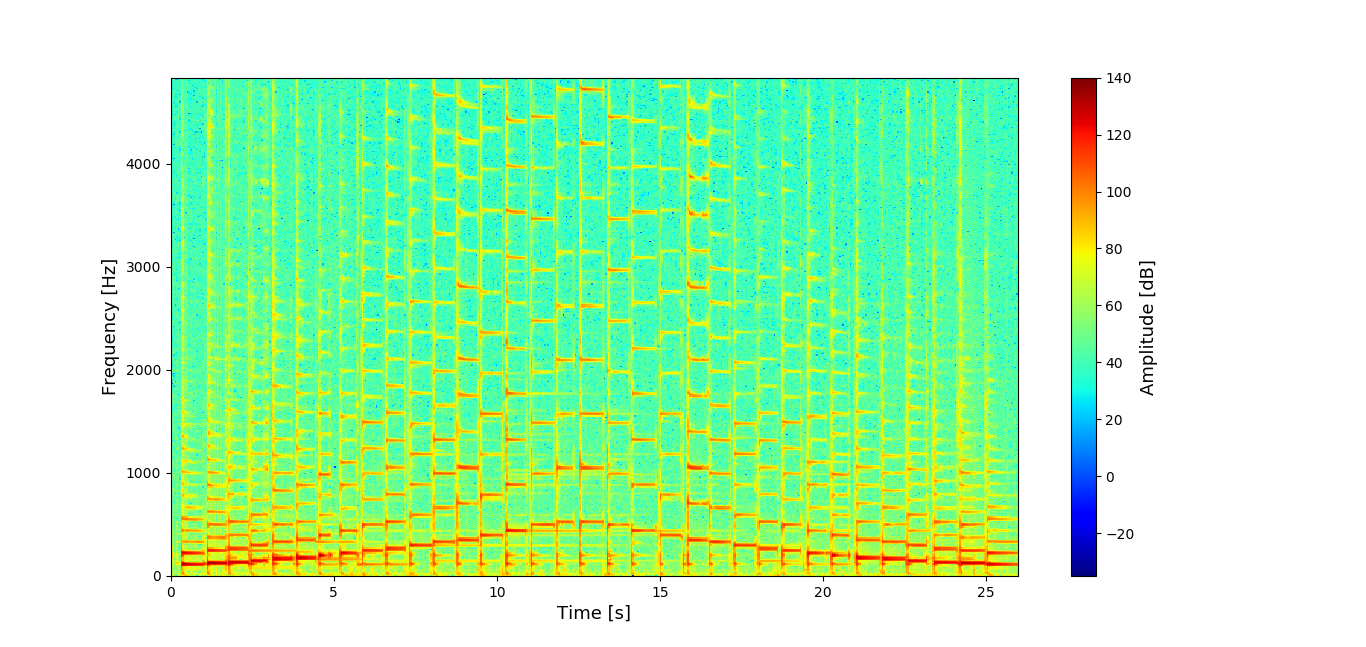
\includegraphics[scale = 0.6]{figures/validation/stft/scale.png}
\caption{Spectrogram of octatonic scale plucking only one string at a time. STFT computed by use of Kaiser window of order $2^{11}$ and $\beta = 4$.}
\label{fig:STFT_test_signal}
\end{figure}